\section{Motivation}
\label{sec:intro:motivation}


\subsection{The Need for Inductive Bias}
As the no-free-lunch theorem for machine learning said,
\cite{baxter2000model,wolpert1995no}, inductive biases that influence
hypothesis selection is necessary to obtain generalization.
\todo{more formal defintion}
\todo{Some easy to follow examples for inductive bias}


\subsection{Where Do Model Get Inductive Biases}
Inductive biases are widely used in the whole history, which can get
from every component of machine learning, from training data, to
optimization algorithm, feature design, even recent neural architures.

\Paragraph{From Training Data} In traditional supervision, models
simplely use training data as inductive bias, such error-based
perceptron model simply update the weight according to the training
data with simple linear models. \todo{history of perceptron, and its
  success}.

\Paragraph{Feature Engineering and Kernel Methods} \todo{Inductve
  biases also can be found in feature engineering, } However, not
every training data are linear seperable, and can be learned by
perceptron. One solution to this kernal-based SVM. The design of
kernel is new inductive.


\Paragraph{Optimization Method} Even in existed computing-heavy and
data-heavy scenarios, inductive biases are widely used in well-known
deep learning techniques. For example, smoothness assumption in
optimization method, such as Stochostic gradient decent, which was
proofed as another inductive bias to have better
generalization. \todo{SGD generalization}


\Paragraph{Neural Artchitecture} What's more, inductive bias are
widely used in modern deep learning architeuctures.  For example,
translation invariance for convolutional neural networks~(CNN) and
pooling, and recurrent assumption of recurrent neural networks~(RNN),
equivariance over permutation for neural graph networks~(GNN), etc.

Towards flexible out-of-distribution and systematic generalization,
the search for appropriate inductive biases are necessary for
bias-variance trade-off when building an NLP system. In this thesis, I
mainly focused on three kinds of inductive biases useful in
deep-learning based NLP system: Structural/Compositional Inductive
Bias, Natural Language supverision as inductive bias, Representation
tuning as inductive bias.

\subsection{Thesis Statement}
\label{ssec:intro:thesis-statemenot}

\todo{rephrase} The use of Compositional inductive bias, Natural
language Supervision as inductive bias, representation tuning as
inductive bias can get beyond what previous component can give.

%
%\subsection{Compositionality in Natural Language}
%
%\begin{figure}[ht]
%\centering
%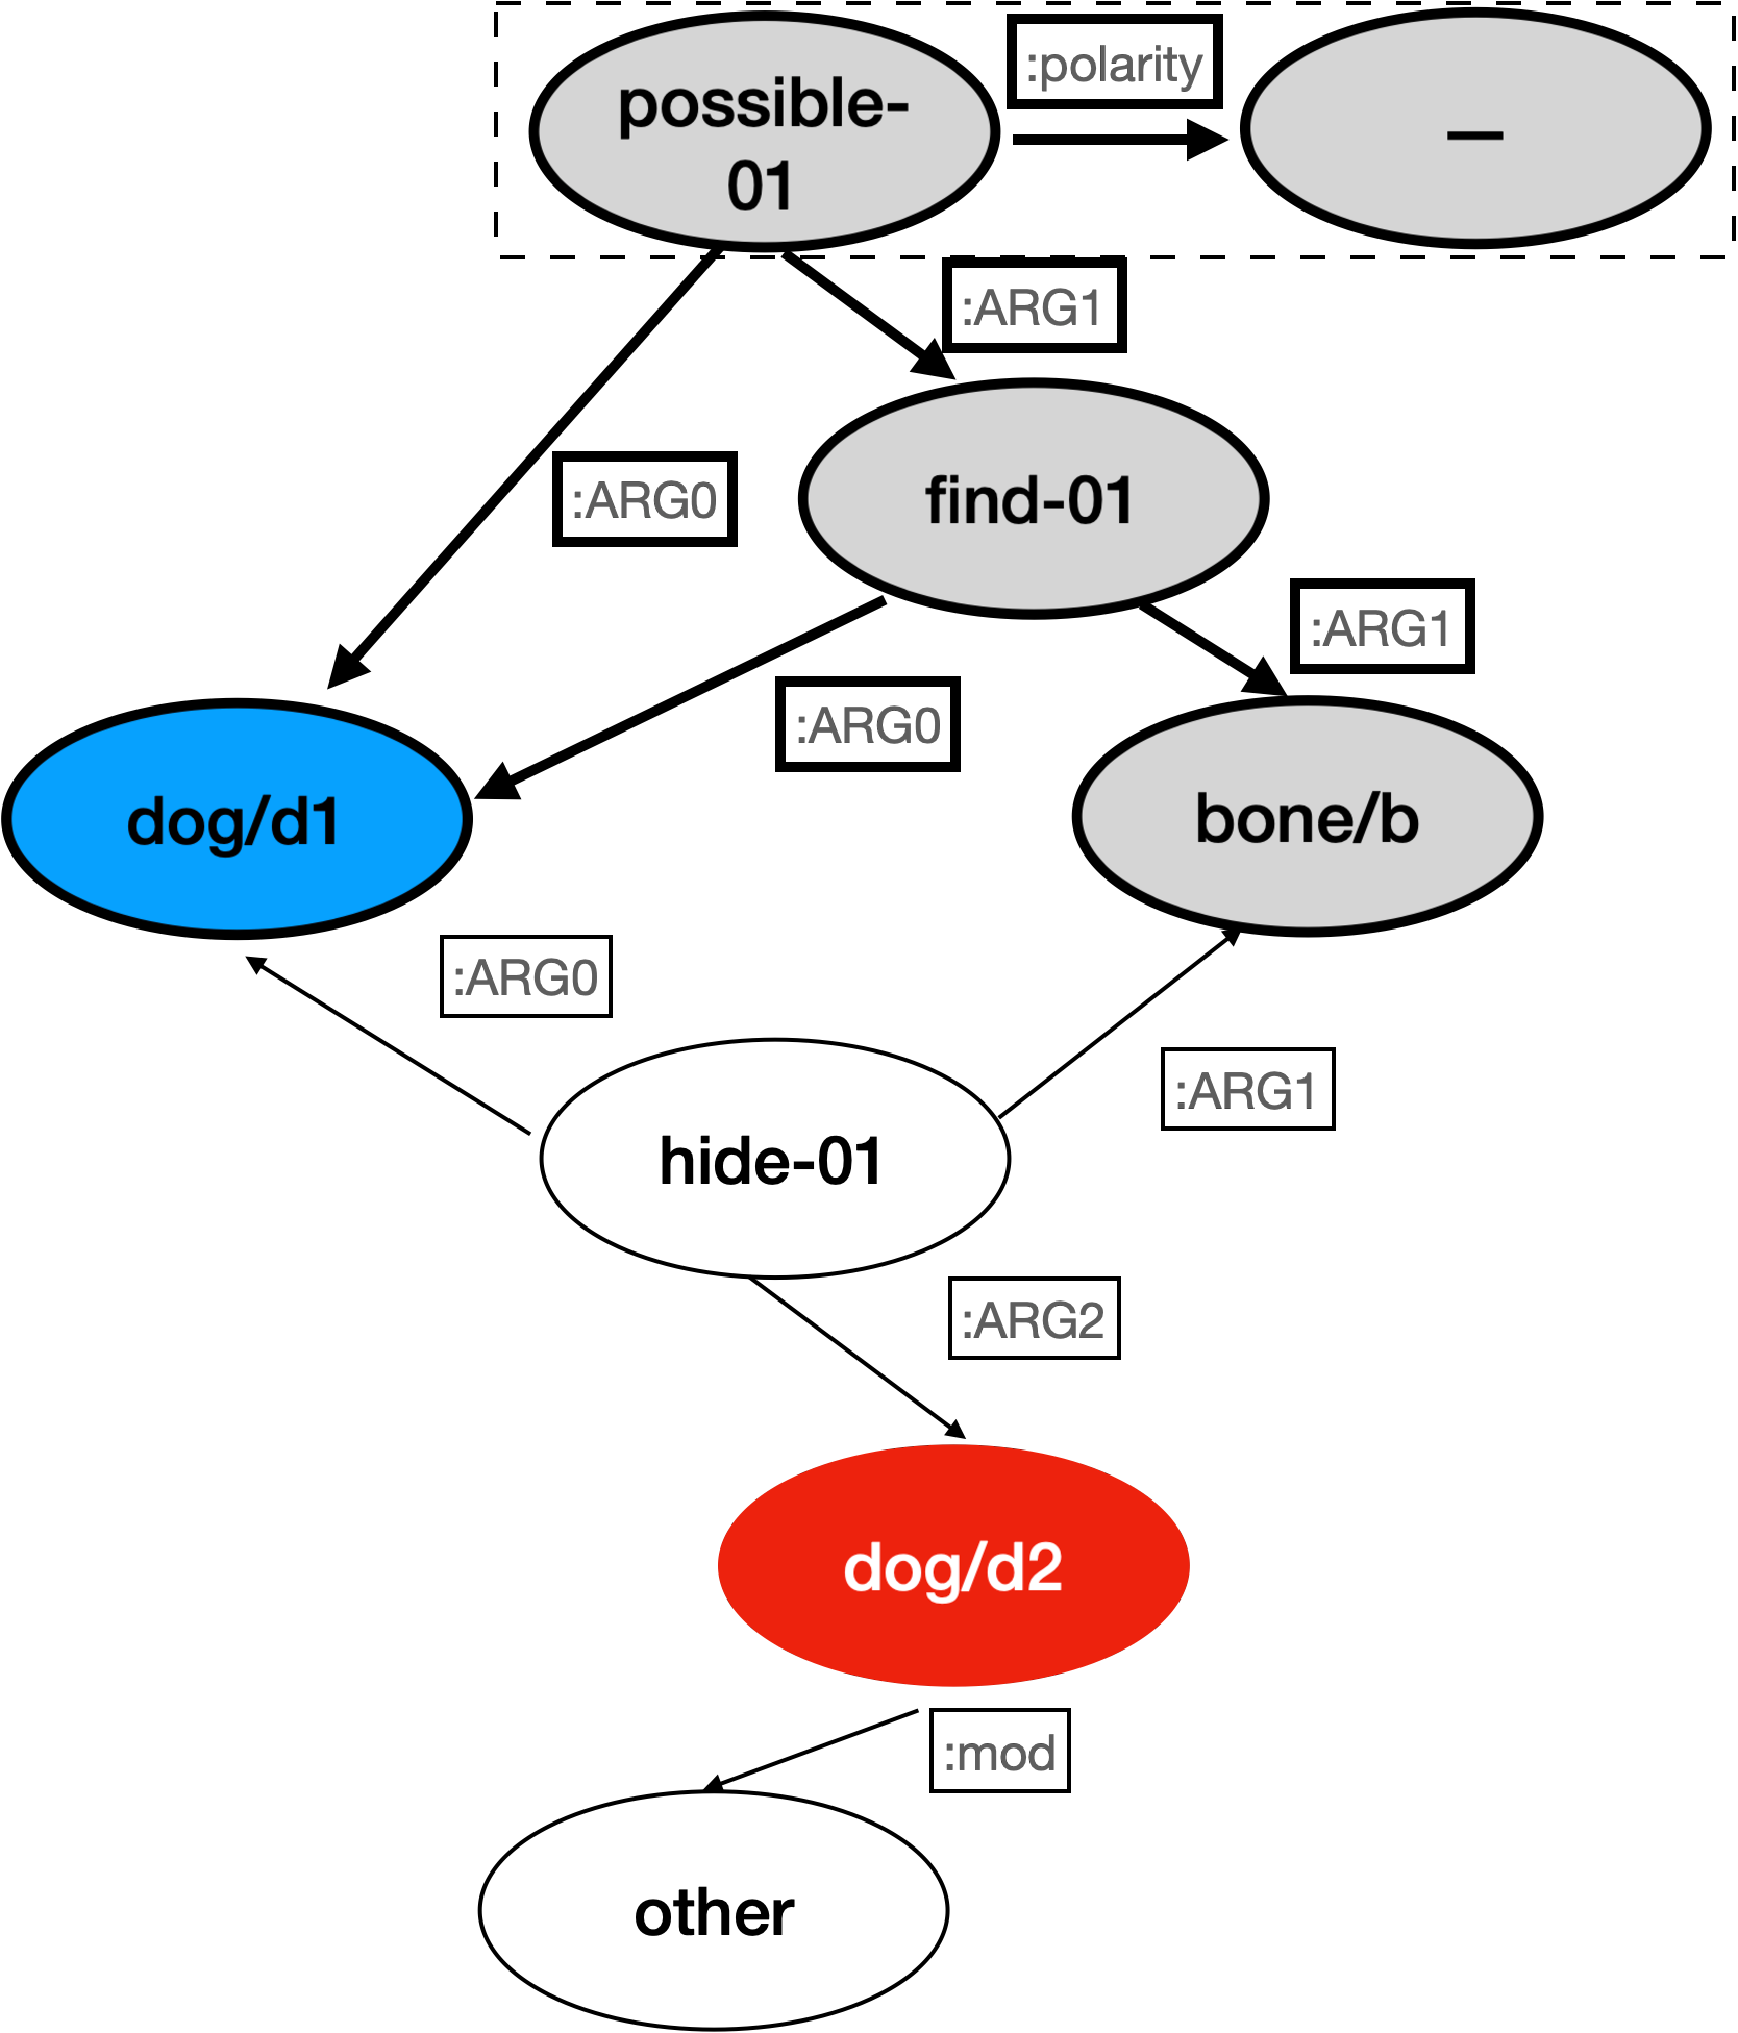
\includegraphics[width=0.45\textwidth]{dog-amr.pdf}
%\caption{\label{fig:intro-example}The AMR graph for the sentence
%  \textit{"The dog cannot find the bone it hid from the other dogs"}}
%\end{figure}
%
%Figure~\ref{fig:intro-example} shows an example of an Abstract Meaning
%Representation~(AMR). It is not difficult to find out how each output
%node~(the ovals represent the nodes/concepts in AMR) can be derived
%from the words in the sentence\footnote{This alignment information is
%  not annotated in AMR training data, which is also happened in many
%  other linguistic structured prediction tasks.}. For example, the
%nodes `find\---01', `bone', `hide\---01' and `other' can be easily aligned
%to the corresponding words in the sentence. However, some ambiguility
%exists when aligning the blue and red `dog' nodes. Additionally, we
%can guess that the subgraph `(possible-01 :polarity -)' in dashed
%rectangle is aligned to the word `cannot'.  Hence, we say
%that the output nodes are \textbf{anchored} to those corresponding
%tokens in the input, and we denote those corresponding input tokens as
%the \textbf{anchors} for the output nodes. Once we find the
%alignments, we can factorize the whole structured prediction problem
%into independent decisions of mapping each candidate anchor into a
%node or a subgraph. Then we connect those predicted nodes or subgraphs
%with edges into a connected graph.  We will formally define this kind
%of decomposition as \textbf{Independent Factorization} in
%\S\ref{ssec:independent-factor}, and study how to leverage this
%inductive bias on different tasks in \S\ref{ssec:sp-anchors}
%
%\begin{figure}[h]
%\centering
%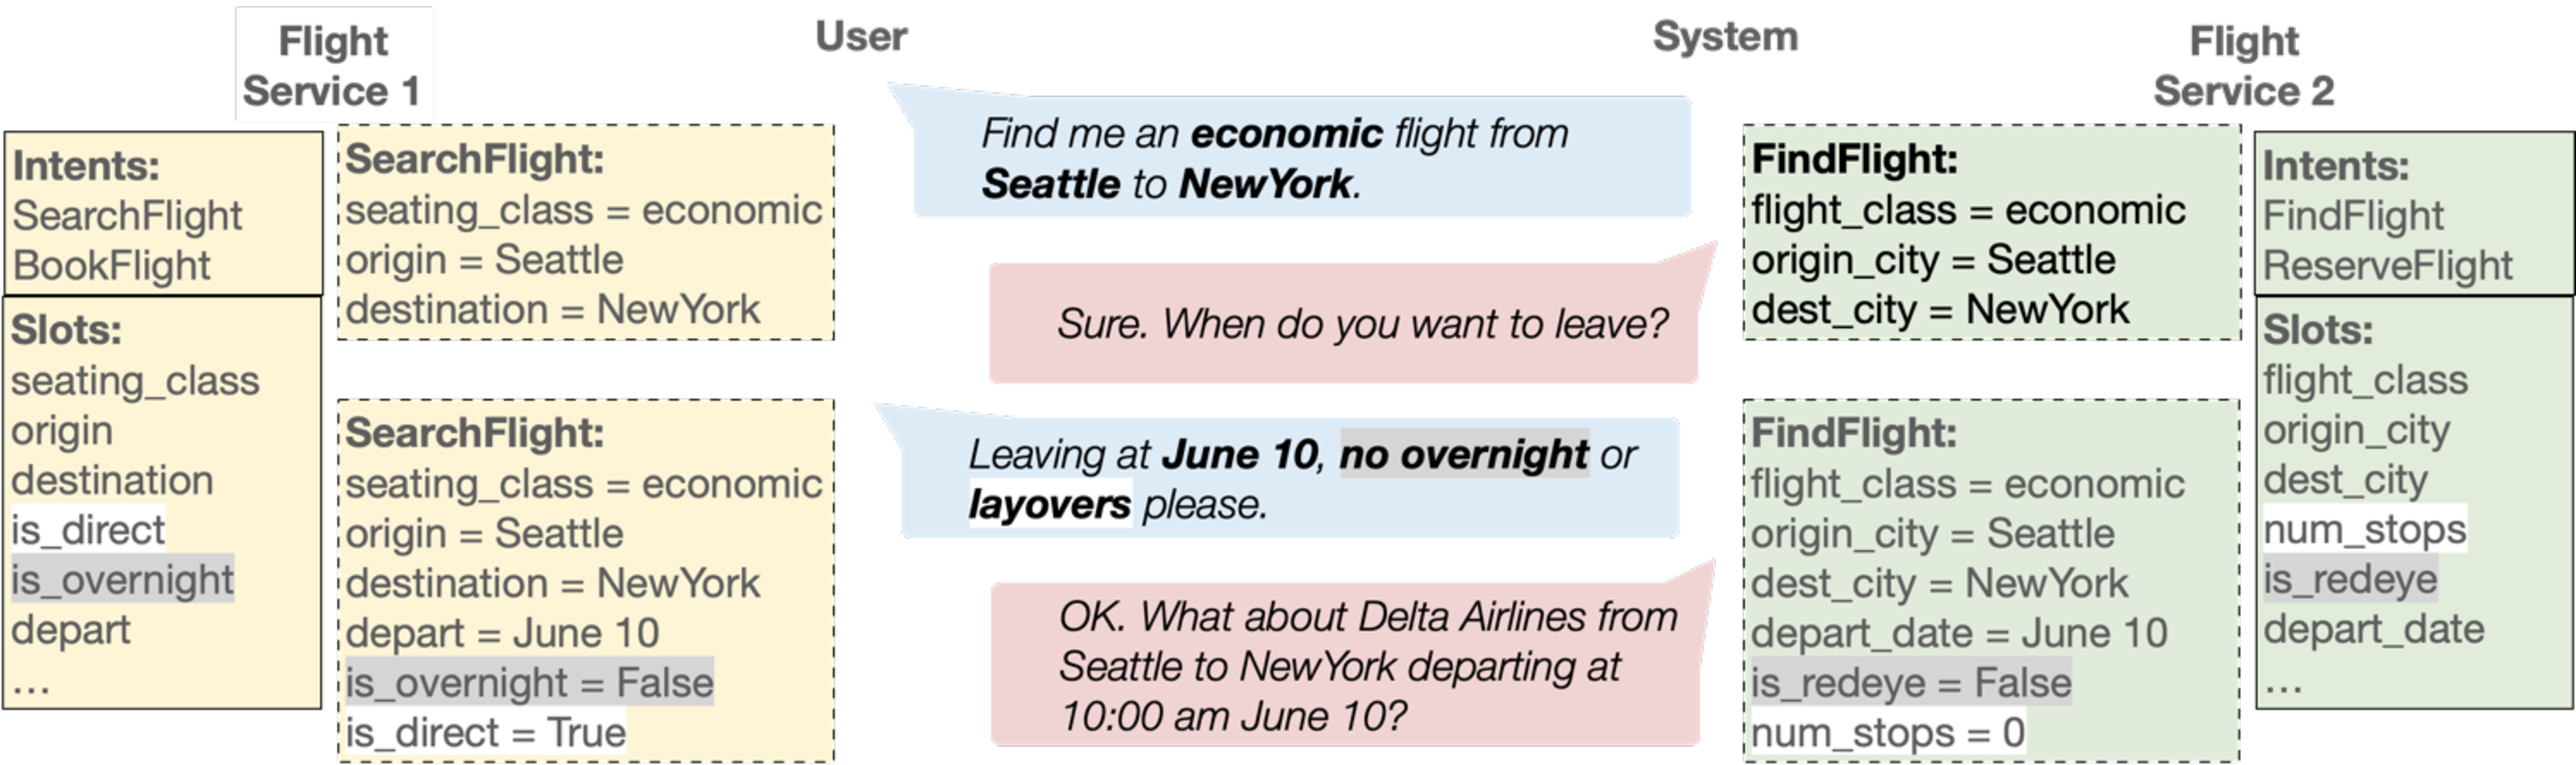
\includegraphics[width=0.92\textwidth]{label-schema-example.pdf}
%\caption{\label{fig:label-example}The heterogeneous services share the
%  overlapping functionalities, but use different slot name, such as
%  "num\_stops" and "direct\_only"}
%\end{figure}
%
%
%\subsection{Compositionality in Symbolic Representation}
%
%According to the principle of compositionality, we believe
%understanding the meaning of each output label will also help for
%structured prediction, especially in a zero-shot domain with
%overlapping functionalities. For example, in the above independent
%assumption for AMR parsing in Figure~\ref{fig:intro-example}, a
%multi-class classification model can be learned to map candidate
%anchors into nodes, then it may generalize well for future
%inference. However, this multiclass classifier will fail when the
%output label set is different from the one seen at training time.  As
%shown in Figure~\ref{fig:label-example}, it shows a dialog state
%tracking example between the user and the system, which is predicting
%the intent/slot frames based on the input dialog and two predefined
%flight services. Assuming we have trained a model on flight service A
%on the left, without retraining the model on new data of service B on
%the right, we hope our model can still generalize well in this
%zero-shot scenarios. These two services share a similar label set, but
%with different names. For example, the service B introduces a new
%boolean slot `direct\_only' which has overlapping meanings with the
%`num\_stops' in service A.  However, the concept of intent and slot
%cannot be richly defined by a single word. Instead, we exploit another
%principle of contextuality to represent the meaning of each label with
%natural language description, and leverage that to generalize to new
%settings in zero-shot learning. We define it as \textbf{Label
%  Representation} in~\S\ref{ssec:label-representation}, and study the
%details in \S\ref{ssec:sgdst}
%
%Finally, besides the representation for individual label, we also
%consider the meaning of the composition in output structures via a
%more general factorization: where each decision on a node and an edge
%will depend on previously predicted partial output. Taking the AMR
%parsing in Figure \ref{fig:intro-example} as an example, instead of
%predicting each node independently, we investigate how to learn a good
%representation for the predicted nodes/edges with bolded borders. Thus
%it empowers the model to learn the inductive biases directly from the
%data, such as their compositional patterns or other constraints. Then
%this structured output representation can guide what to construct next
%without strong independence assumptions or hand-crafted constraints. We
%formally define it as \textbf{Auto-regressive Factorization}
%in~\S\ref{ssec:autoreg-factor}, and study the details in
%\S\ref{sec:proposals}
%
%\subsection{Alignments between Natural Language and Symbolic Representation}

%%% Local Variables:
%%% mode: latex
%%% TeX-master: "../../thesis-main.ltx"
%%% End:
